% Beamer presentation
\documentclass{beamer}
\usepackage[T1]{fontenc}
\usepackage[french]{babel}
\usepackage[french]{datetime2}
\usepackage{multimedia}
\usepackage{hyperref}
\usepackage[backend=biber,style=iso-authoryear,urldate=short]{biblatex}
\addbibresource{bibliography.bib}
\usepackage{tikz}
\usetikzlibrary{arrows.meta,shapes,positioning,calc}
\usepackage{booktabs}

\newcommand{\dateofpresentation}{\DTMdate{2026-08-21}}

\usetheme{Madrid}
\usecolortheme{beaver}

\title{Soutenance de mémoire - Master IS}
\author{David Paulino}
\date{\dateofpresentation}

\begin{document}

\frame{\titlepage}

\begin{frame}
\frametitle{Plan de la présentation}
\tableofcontents
\end{frame}

\section{Introduction}

\subsection{Contexte}
\begin{frame}
\frametitle{Contexte}

Rocket League : un jeu de football avec des voitures.

\vspace{0.2cm}

% Option A : vidéo intégrée (nécessite Adobe Acrobat Reader pour fonctionner)
\begin{center}
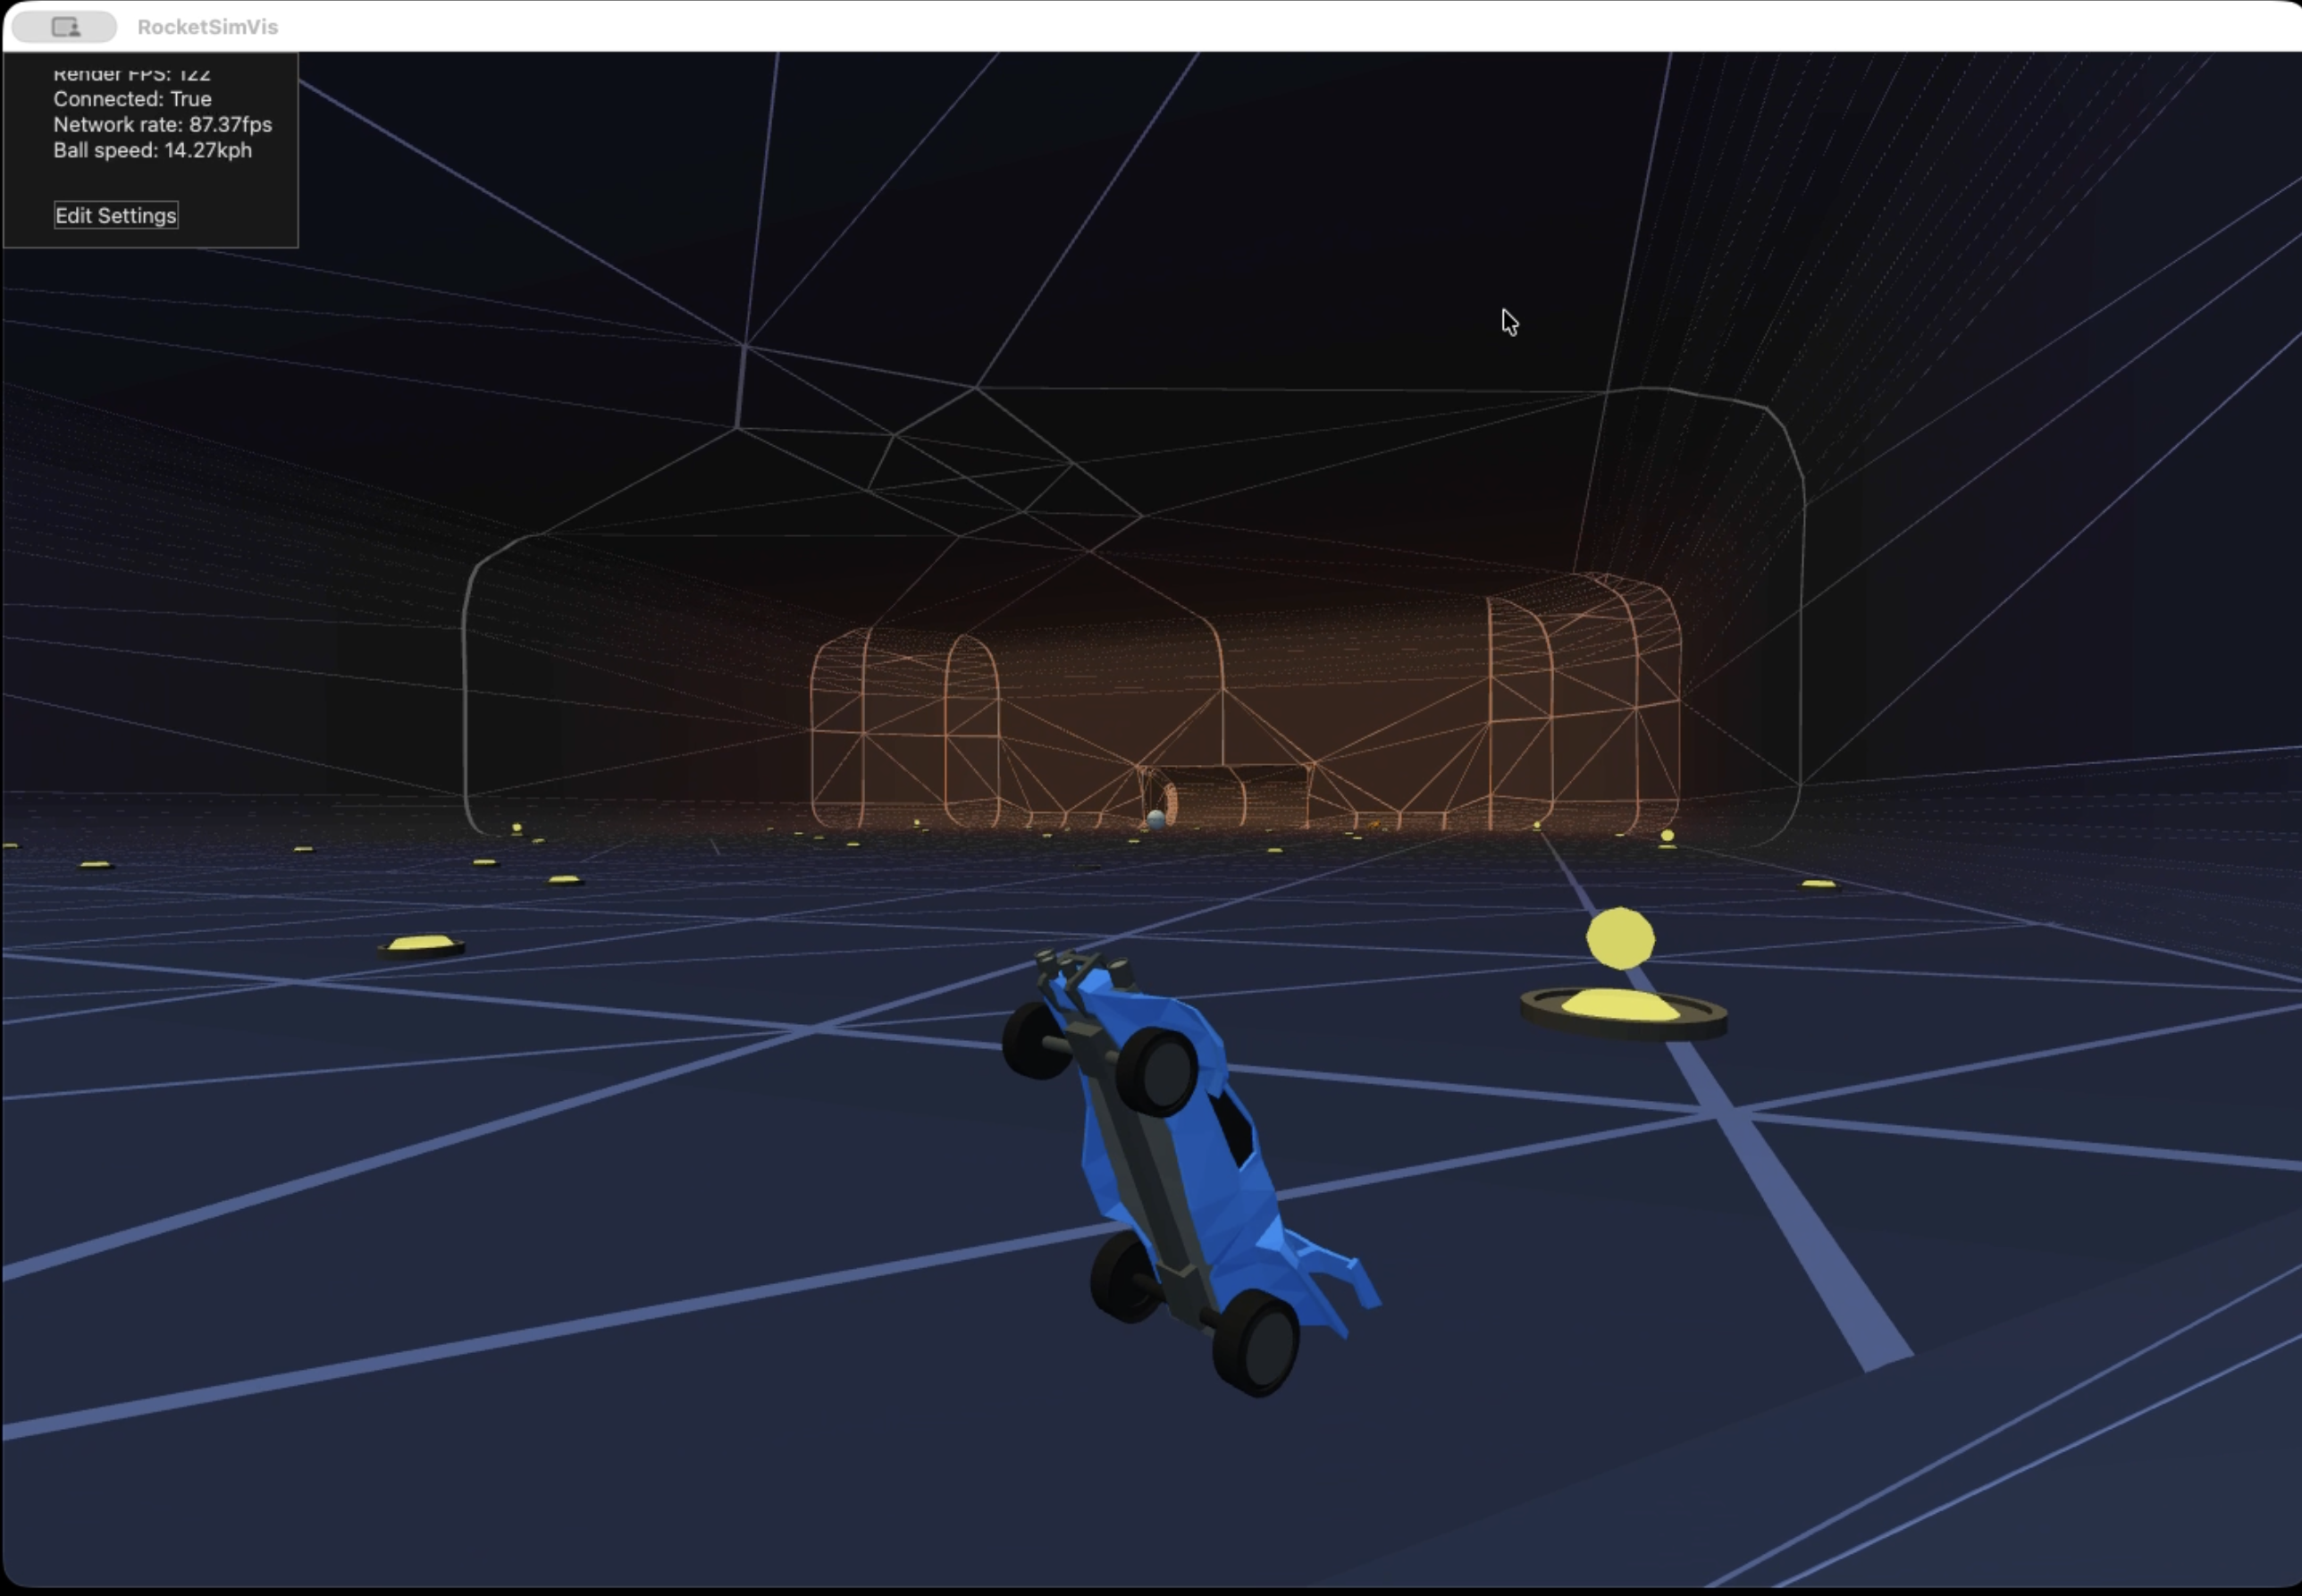
\includegraphics[width=6cm]{img/miniature_agent_not_trained.png}
\end{center}

% Option B (plus sûre) : lien externe à cliquer, ou lancement manuel via VLC
% \href{run:chemin/vers/agent_non_entraine.mp4}{\textbf{Cliquer pour lancer le clip}}

\vspace{0.2cm}

\begin{beamerboxesrounded}[upper=block head,lower=block body]{Question}
    Quelle est la probabilité qu'un agent agissant aléatoirement
    parvienne à marquer un but dans ce jeu ?
\end{beamerboxesrounded}

\vspace{0.2cm}

\centering \textbf{Quasi nulle.}

\end{frame}

\subsection{Problématique}
\begin{frame}
\frametitle{Le problème du \emph{reward sparse}}

Ce phénomène porte un nom : le \textbf{reward sparse} \parencite{narvekarCurriculumLearningReinforcement2020}

\vspace{0.3cm}

\begin{itemize}
    \item Quand l'objectif final n'est atteint que rarement (voire jamais
    au début), l'agent ne reçoit presque aucun signal exploitable.
    \item Résultat : \textbf{absence totale d'apprentissage observable},
    même après des millions de pas d'entraînement.
\end{itemize}

\end{frame}

\begin{frame}
\frametitle{Problématique}

\begin{beamerboxesrounded}[upper=block head,lower=block body]{Problématique}
    Comment mener à bien l'apprentissage par renforcement dans un
    environnement à récompense rare, de la sélection et du réglage
    d'algorithmes standards jusqu'à la conception d'un signal de
    récompense pour un environnement avancé ?
\end{beamerboxesrounded}

\vspace{0.5cm}

\textbf{Deux axes complémentaires :}

\begin{enumerate}
    \item \textbf{Sélection et optimisation des modèles} : quel
    algorithme choisir (DQN, PPO, SAC) selon l'environnement, et
    comment régler ses hyperparamètres ?
    \item \textbf{Construction du signal de récompense} : comment
    densifier un signal rare sans dénaturer la tâche — et quel risque
    cela introduit ?
\end{enumerate}

\end{frame}

\begin{frame}
\frametitle{Démarche en deux phases}

\begin{enumerate}
    \item \textbf{Phase I} — Validation méthodologique sur
    un environnement plus simple \emph{LunarLander} : comparaison DQN / PPO / SAC, optimisation
    Optuna, robustesse multi-seeds.
    \item \textbf{Phase II} — Retour à \textbf{Rocket League} :
    reward shaping et curriculum learning pour surmonter la rareté
    structurelle du signal.
\end{enumerate}

\end{frame}


\section{Fondations minimales}
\subsection{Boucle agent-environnement}
\begin{frame}
\frametitle{Boucle agent-environnement}

% Via tikz. Essayez de montrer la boucle agent-environnement avec un diagramme simple.

\begin{center}
\begin{tikzpicture}[
node distance=3.2cm and 5cm,
>=Stealth,
block/.style={draw, thick, minimum width=3.2cm, minimum height=1.2cm, align=center},
agent/.style={block, ellipse},
env/.style={block, rounded corners=2mm}
]

% --- Nœuds ---
\node[agent] (agent) {Agent};
\node[env, below=of agent] (env) {Environnement};

% --- Flèche Action (Droite) ---
\draw[->, thick] (agent.east) -- ++(1.5,0) |- (env.east)
node[pos=0.5, right, align=left] {action \\ $A_t$};

% --- Flèches de retour (Gauche) ---

% 1. OBSERVATION (Boucle extérieure)
\draw[->, thick] ([yshift=-0.3cm]env.west) -- ++(-3.5,0) |- ([yshift=0.2cm]agent.west);
% Label Observation (toujours à gauche de sa ligne)
\node[left, align=center] at ($(agent.west)+(-3.5, -2.2)$) {observation \\ $O_t$};
\node[below] at ($(env.west)+(-1, -0.3)$) {$O_{t+1}$};

% 2. REWARD (Boucle intérieure)
\draw[->, thick] ([yshift=0.3cm]env.west) -- ++(-3,0) |- ([yshift=-0.2cm]agent.west);
% Label REWARD déplacé à DROITE de sa ligne verticale
\node[right, align=center] at ($(agent.west)+(-3, -2.2)$) {récompense \\ $R_t$};
\node[above] at ($(env.west)+(-1, 0.3)$) {$R_{t+1}$};

% --- Ligne pointillée de transition ---
\draw[dotted, thick] ($(env.west)+(-1.5, 0.8)$) -- ($(env.west)+(-1.5, -0.8)$);

\end{tikzpicture}
\end{center}

\end{frame}

\subsection{Comparaison des algorithmes}
\begin{frame}
\frametitle{Comparaison des algorithmes}

Tableau comparatif des caractéristiques principales de DQN, PPO et SAC.
\begin{center}
\begin{tabular}{|l|ccc|}
\hline
\textbf{Caractéristique} & \textbf{DQN} & \textbf{PPO} & \textbf{SAC} \\
\hline
Paradigme & Off-policy & On-policy & Off-policy \\

Espace d'actions & Discret & Les deux & Continu \\

Sample efficiency & Moyenne & Faible & Élevée \\
\hline
\end{tabular}
\end{center}

\vspace{1cm}

% \begin{beamerboxesrounded}{Note}
%     \footnotesize{
%     PPO par sa nature on-policy est moins sample-efficient car il nécessite de collecter de nouvelles données à chaque mise à jour, tandis que DQN et SAC peuvent réutiliser les expériences passées grâce à leur nature off-policy.}    
% \end{beamerboxesrounded}

\end{frame}

\section{Phase I}
\begin{frame}
    \frametitle{Phase I}
\end{frame}

\section{Phase II}
\begin{frame}
    \frametitle{Phase II}
\end{frame}

% Bibliography
\begin{frame}[allowframebreaks]
\frametitle{Références bibliographiques}
\printbibliography
\end{frame}




\end{document}